\documentclass[palatino]{epflnotes}

\title{Mathematical modeling of DNA}
\author{Guillermo Julián Moreno}
\date{16/17 - Spring semester}

% Additional packages
\usepackage{siunitx}

% --------------------

\begin{document}
\frontmatter
\pagestyle{plain}
\maketitle

\tableofcontents
\mainmatter
% Content

\chapter{Introduction and overview}

\section{Basics of \sectioncaps{DNA}}

\begin{wrapfigure}[12]{R}{0.4\textwidth}
\centering
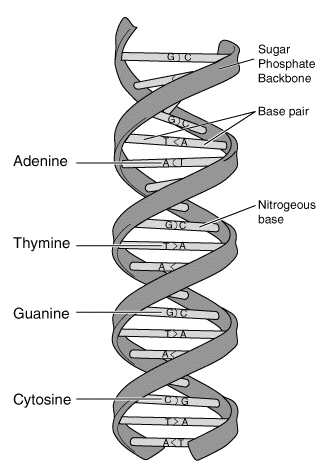
\includegraphics[width = 0.4\textwidth]{img/DNA-structure-and-bases.png}
\caption{Molecular structure of DNA}
\label{fig:DNA}
\end{wrapfigure}

The bases of DNA are denoted by $\mathcal{L} = \set{A,T,C,G}$ with a complementary  rule, where \begin{align*}
\conj{A} &= T &\conj{C} &= G \\
\conj{T} &= A &\conj{G} &= C
\end{align*}

A somewhat interesting fact: the base of the DNA are antiparallel (orientation given by the orientation of the phosphate molecule).

The study of DNA can be separated in its three structures:
\begin{enumerate}
	\item The list of letters $x_i ∈ \mathcal{L} $ for $i = 1, \dotsc, 10^9$ (at least).
	\item The secondary structure is uniform: the double helix.
	\item The tertiary structure relates to the physical properties of the double helix, such as stiffness, which can vary greatly depending on the sequence (up to 25 \%), and its intrinsic shape (the shape of the central line).
\end{enumerate}

Molecular Dynamics simulations of the atoms in DNA and their surrounding medium (water) are considerably expensive, so the focus is in stochastic differential equations for which we can study output probability distribution.

The course-grained model implies simulating not all the atoms but only blocks (sugar, phosphate or whatever is a group for chemists), reducing thus the amount of degrees of freedom.

\section{Course-grained \sectioncaps{DNA} modeling}

We will be interested in models that predict the sequence ground-state structure and flexibility of a sequence. Each configuration space is a vector $\vw ∈ ℝ^N$ and the probability density function $ρ(\vw)$ depends on some constants $Z,β$ and the free energy $U(\vw)$, so that \[ ρ(\vw) = \frac{1}{Z} e^{-βU(\vw)} \]

As the conjugates for each base are clearly defined, we can worry just about the sequence of bases and not the full base pairs. The set of parameters being modeled will by $6n$ intra-basepair and $6(n-1)$ inter-basepair degrees of freedom (see \fref{fig:MovementsDNA}), so a total of $N = 12n - 6$ degrees of freedom for a sequence of $n$ basepairs.

For the cgDNA model, the free energy is approximated as a quadratic form \[ U(\vw)= \frac{1}{2} (\vw - μ) · \mK · (\vw -μ)\] with $μ = μ(S) ∈ ℝ^N$ being the ground state configuration and $\mK = \mK(S) ∈ ℝ^{N×N}$ being the ground-state stiffness, represented by a symmetric and positive-definite matrix.

Of course, the question is how to get those ground states $μ, \mK$ from the sequence $S$ you are studying. The main assumption is that those states are only affected by junction and intra-basepair interaction energies, as shown in \fref{fig:MovementsDNA}, and that the groudn state is the one with minimum energy. During these lectures we will introduce this model and do more things.

\begin{figure}[tbp]
\centering
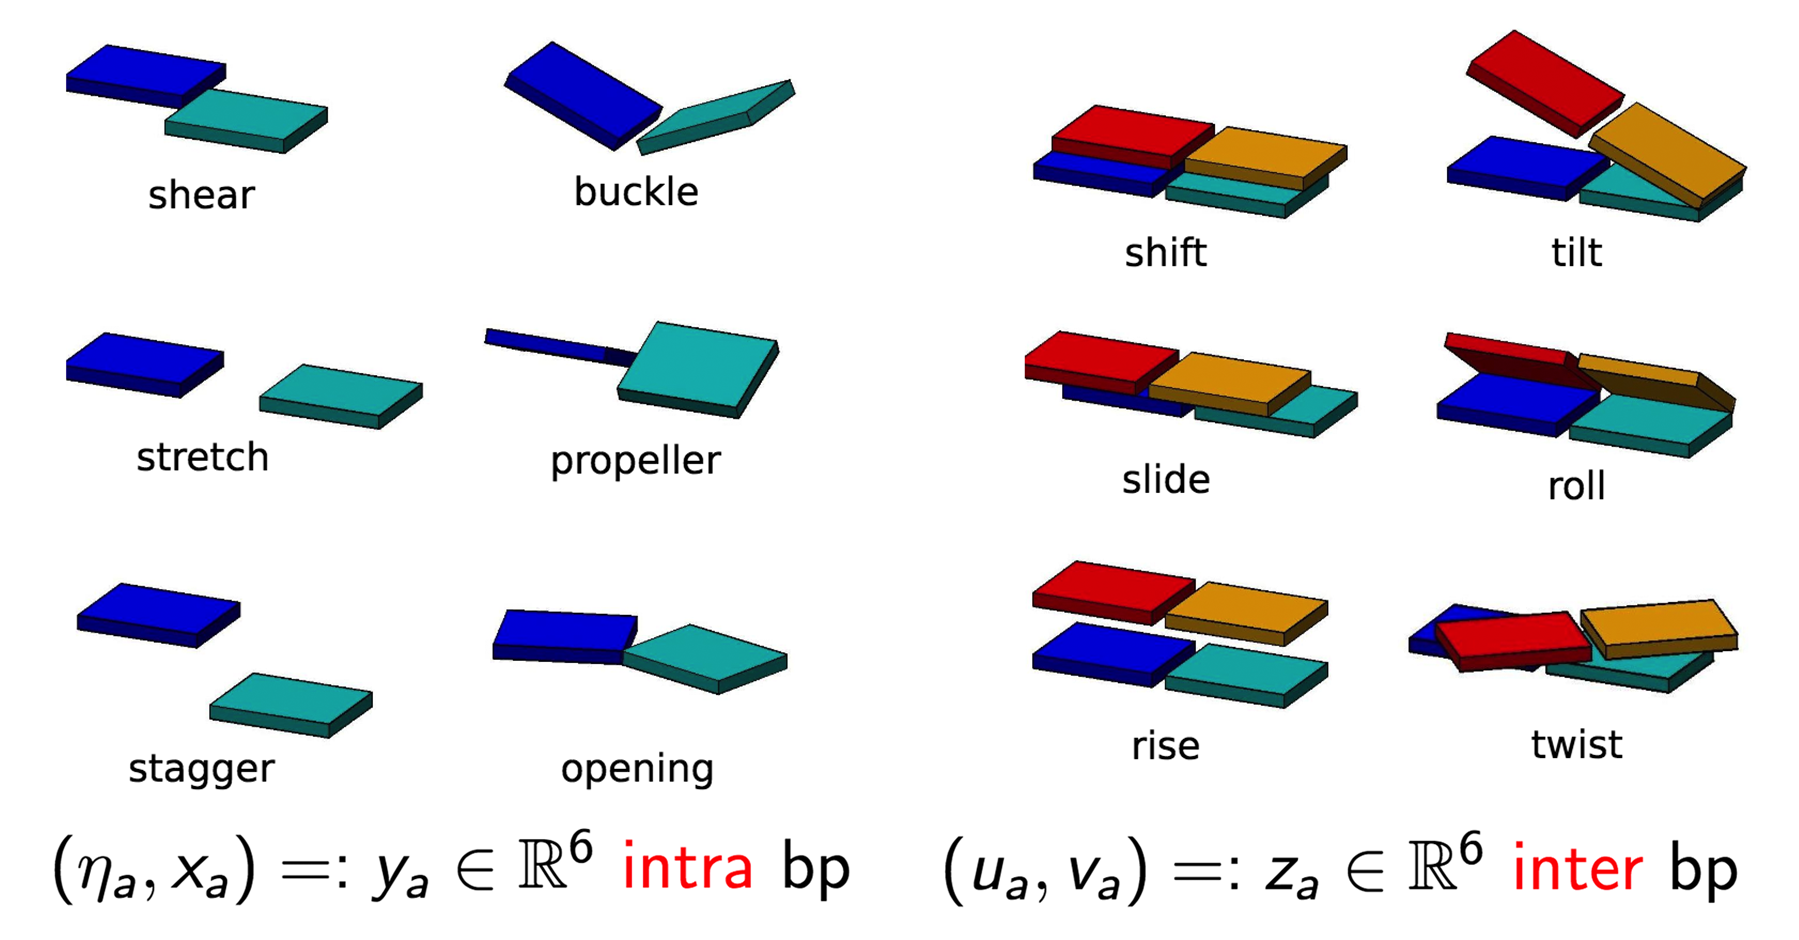
\includegraphics[width=0.8\textwidth]{img/movementsDNA.png}
\caption{Interpair and intrapair interactions}
\label{fig:MovementsDNA}
\end{figure}

\chapter{cgDNA model}

We will consider the coarse-grain model of DNA in which each base on each strand is modeled as an independent rigid body. First, we will define what we mean by an independent rigid body and what mathematical tools do we need to deal with them, and then we will go straight to the modeling.

\section{Rigid body framings: $SE(3)$}

\section{Modeling of \sectioncaps{DNA} sequences}

\subsection{Framing of the base pairs}

\begin{figure}[hbtp]
\centering
\inputtikz{WatsonCrickModel}
\caption{Basic nomenclature in DNA sequences, with $X_i ∈ \set{T,A,C,G}.$}
\label{fig:WatsonCrickStrand}
\end{figure}

We consider a DNA molecule to be identified, as seen in \fref{fig:WatsonCrickStrand}, with a sequence of bases $\set{X_1, \dotsc, X_n}$ along one strand (one side of the helix for us non-biologists), listed in the $5'$ to $3'$ direction (that is, bottom to top). Each base pair is denoted by $(X, \conj{X})_i$, and we will ignore the atoms forming the sugar-phosphate backbones.


For each one of the base pairs we will consider two rigid body motions. One will be referring to the movement between one base and its corresponding one in the other strand, and the other one will model the rigid body motion from one strand to the next one.

\begin{figure}[hbtp]
\centering
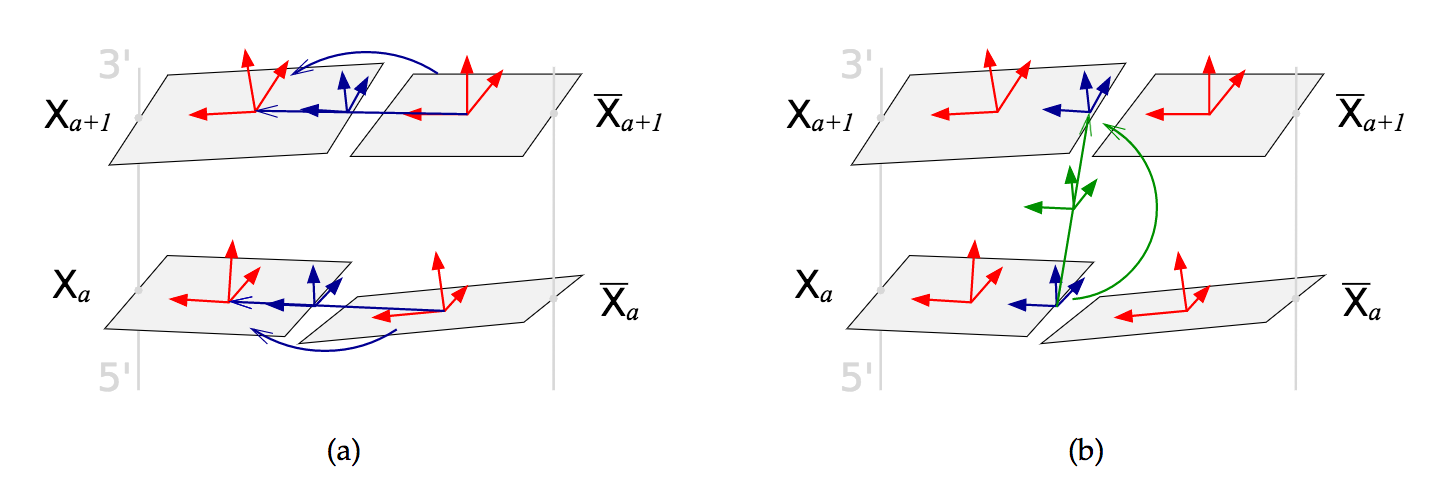
\includegraphics[width=0.8\textwidth]{img/CrickWatson.png}
\caption{A schematic illustration of the base (red), base-pair (blue), and junction (green) frames for an isolated base-pair step.}
\end{figure}

% Missing some week 2 and week 3 material here

What we have then is that, for each level $i$ in the sequence, we have the positions and rotations $R_i^+ ≝ (\mR_i^+, \vr_i^+) ∈ SE(3)$ and $R_i^- ≝ (\mR_i^-, \vr_i^-) ∈ SE(3)$ of both bases (Watson and Crick strands respectively). We are interested in simplifying this and having a parametrization in which we can consider separately between the inter and intra basepair motions.

We will introduce then the position/rotation of the basepair as $R_i ≝ (\mR_i, \vr_i)$ defined as the ``average'' of $R_i^+$ and $R_i^-$. For the rotation that is half the rotation from $\mR_i^+$ to $\mR_i^-$, and for the position that is the midpoint between $\vr_i^+$ and $\vr_i^-$:
\begin{align*}
\mR_i &= \mR_i^- \sqrt{\mQ_i} \\
\vr_i &= \frac{\vr_i^+ + \vr_i^-}{2}
\end{align*} with $\mQ_i = \trans{(\mR_i^-)} \mR_i^+$ the rotation between bases.

In a similar way we can write the displacement between pairs based on the junction frame, defined as \begin{align*}
\mJ_i &= \mR_i \sqrt{\mP_i} \\
\vj_i &= \frac{\vr_i + \vr_{i+1}}{2}
\end{align*} with $\mP_i = \trans{\mR_i} \mR_{i+1}$ being the rotation between base-pair frames.

We can keep on simplifying further: we can get rid of global rotations and translation of the full DNA sequence if we consider not a series of frames and positions but a series of movements and rotations to get from one basepair to another instead.

This leads us to define a set of DNA coordinates starting from an initial assumed configuration $R_1 = (\mop{Id}, \vec{0})$, the intra-pair rigid body motions $Q_i ≝ (\mQ_i, \vq_i)$ and the inter-pair ones $P_i ≝ (\mP_i, \vp_i)$. These allow the calculation of each base position and frame by a recursion relation:
\begin{align*}
\begin{pmatrix} \mR_{i+1} & \vr_{i+1} \\ 0 & 1 \end{pmatrix} &=
	\begin{pmatrix} \mR_i & \vr_i \\ 0 & 1 \end{pmatrix}
	\begin{pmatrix} \mP_i & \sqrt{\mP_i} \vp_i \\ 0 & 1 \end{pmatrix} \\
\begin{pmatrix} \mR_i^+ & \vr_i^+ \\ 0 & 1 \end{pmatrix} &=
	\begin{pmatrix} \mR_i^{-} & \vr_i^- \\ 0 & 1 \end{pmatrix}
	\begin{pmatrix} \mQ_i & \sqrt{\mQ_i} \vq_i \\ 0 & 1 \end{pmatrix}
\end{align*}

The displacements $\vp_i$ and $\vq_i$ can be simply calculated from that relation of recurrence as \begin{align*}
\vp_i &= \trans{\sqrt{\mP_i}} \trans{\mR_i} (\vr_{i+1} - \vr_{i}) = \trans{\mJ} \underbracket{(\vr_{i+1} - \vr_{i})}_{Δ\vr_i} \\
\vq_i &= \sqrt{\trans{\mQ_i}} \trans{(\mR_i^-)} (\vr_i^+ - \vr_i^-) = \mR_i \underbracket{(\vr_i^+ - \vr_i^-)}_{δ\vr_i}
\end{align*}

That is, $\vp_i$ and $\vq_i$ are, respectively, the inter-pair and intra-pair displacements $Δ\vr_i$ and $δ\vr_i$ in the corresponding frames $\mJ_i$ and $\mR_i$. This definition will also be helpful if at some point in the future we want to ``reverse'' the sequences, as we are setting reference frames that will not depend on the direction we traverse the sequence in.

We can improve this a little bit more. Both $\mQ_i$ and $\mP_i$ are in $SO(3)$, that is, we have 9 entries each but there are only 3 independent parameters for each rotation (the ones described in \fref{fig:MovementsDNA}).

So, we need to get to a minimal set of coordinates by introducing the Cayley transform. Provided that neither $\mP_i$ or $\mQ_i$ are close to rotations by π, there exists an unique mapping \begin{align*}
\appl{\cayley}{SO(3) & }{ℝ^3} \\
\mP_i &\longmapsto \vu_i \\
\mQ_i &\longmapsto \veta_i
\end{align*}

The question is, however, in which frame are the components of $\vu_i$. The available optionsare $\mR_i, \mJ_i$ or $\mR_{i+1}$. Similarly, we need to know in which frame are the components of $\veta_i$, as we can have $\mR_i^-$ or $\mR_i$ or $\mR_i^+$.

A nice property of Cayley vector is that it has the same coordinates for all the frames along the rotation, so the answer is that the components of $\vu_i$ are the same in $\mR_i, \mJ_i$ and $\mR_{i+1}$ as it represents the rotation from $\mR_i$ to $\mR_{i+1}$ with $\mJ_i$ being the rotation at the midpoint. The same applies to $\veta_i$.

Finally, we can explain the cgDNA model configuration coordinates. This has, for $N$ base pair ligomer a vector $\vw ∈ ℝ^{12N - 6}$ as $\vw = (\vy_1, \vz_1, \dotsc, \vz_{N-1}, \vy_N)$ where $\vz_i ∈ ℝ^6$ are the inter pair rotations and translations and $\vy_i ∈ ℝ^6$ are the intra pair rotations and translations with the rotations as a Cayley vector.

\subsubsection{Inversion of sequences}

We briefly consider here the transformation rule for inversion of a sequence. We will prove later in detail, but if $\vw$ are the coordinates for a specific configuration of the DNA fragment for one choice of the Watson strand then the coordinates $\bar{\vw}$ for the configuration in the reverse sense are $\bar{\vw} = \mE_{2N - 1} \vw$ where \[ \mE_{2N-1} = \begin{pmatrix} 0 & \cdots & \mE \\ \vdots &\iddots & \vdots \\ \mE & \cdots & 0 \end{pmatrix} \] with $\mE ∈ ℝ^{6×6}$ just $-1, +1, +1, -1, +1, +1$ on the leading diagonal.

\subsection{Energy of the DNA sequence configuration}

The cgDNA model predicts a probability density function $ρ(\vw; S, P)$ for each configuration $\vw$, depending on the sequence $S$ and the parameter set $P$. For convenience, $S$ and $P$ may be suppressed anywhere in notation.

The assumption is that the PDF is going to be related to an energy distribution, with lower energy states being more probable. Thus, the formula will be something like \[ ρ(\vw; S, P) = \frac{1}{Z} e^{- U(\vw; S, P)} \] where $Z$ is the normalizing constant and $U$ will be quadratic polynomial in $\vw$.


So $U$ is going to look like

In order to derive the expression for the energy, we assume that the energy of a DNA configuration depends on the energy between bases in a pair and on the cross-junction interaction energies. We assume that all those interactions are quadratic and have minimum-energy states $\hat{\vy}_i$ and $\hat{\vx}_j$ so the energy takes on a form like this: \[ 2U(\vw) = \sum_{i = 1}^N (\vy_i - \hat{\vy}_i) · \mK_{i}^{BP} (\vy_i - \hat{\vy}_i) + \sum_{j=1}^{N-1} (\vx_j - \hat{\vx}_j) \mK^J_j (\vx_j - \hat{\vx}_j)\] which represent respectively the sum of something over basepairs and sum over junctions, and where where $\vx_j = (\vy_j, \vz_i, \vy_{i+1})$. Also $\mK_i^{BP} ∈ ℝ^{6×6}$ and $\mK_{j}^J ∈ ℝ^{18 × 18}$ are symmetric.

It can be shown that this expression is simplifiable to a single quadratic form if we get rid of constant terms. This expression is
\[ U(\vw) = \frac{1}{2} (\vw - \vmu(S)) \mK(S) (\vw - \vmu(S)) \] where $\mK(S) ∈ ℝ^{(12N - 6) × (12N - 6)}$ is a symmetric and positive-definite matrix. Also, $\vmu(S) ∈ ℝ^{12N-6}$ will be the ground-state vector.

An interesting thing about this expression is that, while we have built a model based on local interactions, the ``competition'' between ground stats $\hat{\vy}_i$ and $\hat{\vx}_i$ for each of the different energies will imply non-local sequence dependence\footnote{One can show it doing some computations and linear algebra. But it's not interesting.}.

\appendix

\chapter{Exercises}
% -*- root: ../MathModelingDNA.tex -*-

\backmatter
\printindex
\end{document}
